\chapter{METODOLOGI PENELITIAN}

\section{Alat dan Bahan}
	Alat dan bahan yang digunakan pada penelitian ini terbagi atas perangkat keras dan perangkat lunak yang akan dijelaskan seperti berikut.

	\subsection{Perangkat Keras}
	Perangkat keras terdiri dari sebuah FPGA board yang digunakan sebagai
	media inferensi model CNN serta sejumlah pheripheral meida untuk
	melakukan \emph{streaming meida} untuk pengambilan data. Detail mengenai
	perangkat keras yang digunakan terdapat pada daftar berikut.

		\vspace{-0.5cm}

		\begin{enumerate}[a.]
		\begin{singlespace}
		\itemsep0em
			\item Digilent Arty A7-100T,
			\item OV7670,
			\item \emph{VGA Pmod Digilent},
			\item \emph{USB},
			\item 14 Jumper \emph{Male-Female},
		\end{singlespace}
		\end{enumerate}

	\subsection{Perangkat Lunak}
	Perangkat lunak yang digunakan selama proses pengembangan mencakup
	lingkungan kerja dan lingkungan uji. Detail mengenai perangkat
	lunak yang digunakan terdapat pada daftar berikut.

		\vspace{-0.5cm}

		\begin{enumerate}[a.]
		\begin{singlespace}
		\itemsep0em
				\item Software VIVADO,
				\item Linux Operating System,
				\item Python,
				\item Kaggle,
				\item Verilog Icairus,
				\item Visual Studio Code.
		\end{singlespace}
		\end{enumerate}

\section{Rancangan Sistem}
    \subsection{Rancangan Umum Sistem}
		\begin{figure}[H]
		\centering
		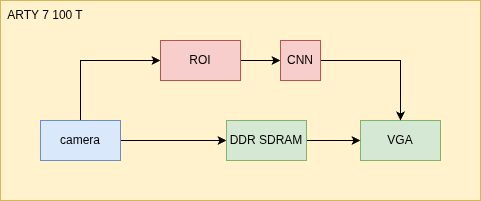
\includegraphics[width=0.75\textwidth]{gambar/rancangan-umum-sistem.png}
		\caption{Rancangan Umum Sistem}
		\label{fig:rancangan-umum-sistem}
	\end{figure}
	DDR SDRAM digunakan sebagai \emph{frame buffer} agar
	data citra dari kamera dan data yang akan ditampilkan
	ke VGA dapat dipisahkan secara lebih stabil. Jalur
	kamera, DDR, dan VGA berperan sebagai sistem akuisisi
	dan tampilan citra, sedangkan jalur ROI dan CNN
	berperan sebagai sistem klasifikasi. Pemisahan ini
	dilakukan agar proses inferensi CNN tidak harus
	dilakukan pada seluruh frame, melainkan hanya pada
	area tertentu yang dianggap relevan. Dengan demikian,
		beban komputasi dapat dikurangi tanpa menghilangkan
		fungsi utama sistem sebagai sistem klasifikasi citra
		berbasis FPGA.

	\subsection{Dataset}
		Dataset yang digunakan pada penelitian ini adalah dataset MNIST yang diperoleh
		dari Kaggle \cite{KaggleMNISTDataset}. Dataset MNIST berisi citra angka
		tulisan tangan dari digit 0 sampai 9. Setiap citra memiliki ukuran
		$28 \times 28$ piksel dan direpresentasikan dalam bentuk \emph{grayscale}.
		Karakteristik ini sesuai dengan kebutuhan penelitian karena rancangan CNN
		menggunakan satu kanal input dan menghasilkan 10 kelas keluaran, yaitu
		kelas digit 0 sampai 9. Dengan demikian, dataset MNIST dapat digunakan
		sebagai dasar pelatihan dan pengujian model sebelum parameter model
		dikonversi ke format \emph{fixed-point} untuk implementasi pada FPGA.

		Pemilihan MNIST juga dilakukan karena ukuran citra relatif kecil dan struktur
		datanya sederhana, sehingga sesuai untuk tahap validasi awal akselerator CNN
		berbasis FPGA. Ukuran input $28 \times 28$ memungkinkan proses konvolusi,
		pooling, dan \emph{fully connected} diuji tanpa membutuhkan kapasitas memori
		dan resource komputasi yang terlalu besar. Hal ini penting karena fokus
		penelitian bukan hanya pada akurasi model, tetapi juga pada keterlaksanaan
		implementasi hardware, penggunaan resource FPGA, latensi inferensi, serta
		perbandingan hasil komputasi antara Python dan Verilog.

    \subsection{Rancangan Arsitektur CNN}
	Arsitektur CNN yang digunakan pada penelitian ini
	dirancang sebagai model klasifikasi citra berukuran
	kecil agar sesuai dengan keterbatasan sumber daya
	pada FPGA. Input model berupa citra grayscale
	berukuran $28 \times 28$ piksel yang diperoleh dari
	hasil pemrosesan ROI. Model CNN dikembangkan
	terlebih dahulu menggunakan Python sebagai model
	acuan sebelum parameter bobot dan biasnya dipindahkan
	ke implementasi Verilog. Penggunaan CNN dipilih
	karena metode ini mampu mengekstraksi fitur citra
	secara bertahap melalui operasi konvolusi, aktivasi,
	dan pooling \cite{Goodfellow2016DeepLearning, Lecun1998GradientBasedLearning}.

	Secara umum, model terdiri dari tiga blok konvolusi
	dan dua lapisan \emph{fully connected}. Blok pertama
	menerima satu kanal input dan menghasilkan 8 kanal
	fitur. Blok kedua menghasilkan 16 kanal fitur,
	sedangkan blok ketiga menghasilkan 32 kanal fitur.
	Setiap blok konvolusi menggunakan kernel $3 \times 3$
	yang diikuti oleh fungsi aktivasi ReLU dan proses
	\emph{max pooling}. Setelah tahap ekstraksi fitur
	selesai, hasil akhir diproses oleh lapisan
	\emph{fully connected} untuk menghasilkan 10 nilai
	keluaran yang merepresentasikan kelas prediksi.
	Pada implementasi hardware, tahap \emph{softmax}
	tidak digunakan karena proses klasifikasi cukup
	dilakukan dengan membandingkan nilai keluaran
	terbesar menggunakan \emph{argmax}.

	Arsitektur ini dipilih karena memiliki jumlah
	parameter yang relatif kecil, tetapi tetap mampu
	merepresentasikan proses ekstraksi fitur CNN secara
	bertingkat. Selain itu, ukuran model yang tidak
	terlalu besar membuatnya lebih memungkinkan untuk
	diimplementasikan pada FPGA dengan komputasi
	\emph{fixed-point}. Parameter model berupa bobot
	dan bias disimpan sebagai data konstan pada memori
	internal, sehingga proses inferensi dapat dilakukan
	secara langsung oleh rangkaian hardware tanpa
	memerlukan proses pelatihan ulang di dalam FPGA.

    \subsection{Rancangan Representasi Fixed-Point}
	Representasi numerik pada rancangan akselerator CNN dibuat menggunakan format
	\emph{fixed-point} 16-bit. Pemilihan format ini dilakukan karena model CNN pada
	tahap pelatihan masih menggunakan \emph{floating-point}, sedangkan implementasi
	pada FPGA lebih sesuai apabila operasi aritmetika direalisasikan dalam bentuk
	bilangan integer atau \emph{fixed-point}. Operasi \emph{floating-point} membutuhkan
	rangkaian aritmetika yang lebih kompleks dan dapat meningkatkan penggunaan
	resource, terutama pada operasi perkalian dan akumulasi yang muncul berulang pada
	layer konvolusi dan \emph{fully connected}. Oleh karena itu, parameter model hasil
	pelatihan, seperti bobot dan bias, dikonversi terlebih dahulu ke dalam format
	\emph{fixed-point} sebelum dimasukkan ke dalam memori parameter pada Verilog
	\cite{Zhang2015OptimizingCNNFPGA,Solovyev2019FixedPointCNN}.

	Pada penelitian ini, representasi \emph{fixed-point} menggunakan format Q2.14,
	yaitu format 16-bit bertanda dengan dua bit untuk bagian integer termasuk bit
	tanda dan 14 bit untuk bagian fraksi. Dengan konfigurasi tersebut, nilai
	\emph{floating-point} dikalikan dengan faktor skala $2^{14}$, kemudian dibulatkan
	dan dibatasi agar tetap berada pada rentang bilangan bertanda 16-bit. Format
	Q2.14 memiliki rentang nilai real sekitar $[-2, 2)$ dengan resolusi sebesar
	$2^{-14}$. Pemilihan format ini dilakukan karena nilai parameter model, baik
	bobot maupun bias, tidak keluar dari rentang $-2$ sampai $2$, sehingga dua bit
	bagian integer sudah cukup untuk menampung rentang nilai parameter.

	Pemakaian 14 bit fraksi penting karena nilai bobot CNN umumnya berada pada
	rentang kecil, sehingga dibutuhkan resolusi pecahan yang cukup halus agar
	informasi parameter tidak banyak hilang setelah proses kuantitasi. Dengan
	memprioritaskan bit untuk bagian fraksi, perubahan kecil pada parameter masih
	dapat direpresentasikan dengan lebih baik dibandingkan apabila lebih banyak
	bit dialokasikan untuk bagian integer. Secara umum, proses konversi dari nilai
	real $x$ ke representasi \emph{fixed-point} 16-bit dapat dituliskan sebagai
	berikut.

	\begin{equation}
	q_{16} =
	\operatorname{clip}
	\left(
	\operatorname{round}(x \cdot 2^F),
	-2^{15},
	2^{15}-1
	\right)
	\label{eq:fixed-point-1}
	\end{equation}

	\begin{equation}
	\hat{x}_{16} = q_{16} \cdot 2^{-F}
	\label{eq:fixed-point-2}
	\end{equation}

	Pada Persamaan \ref{eq:fixed-point-1} dan \ref{eq:fixed-point-2}, fungsi
	$\operatorname{round}(\cdot\cdot\cdot)$ digunakan untuk membulatkan hasil perkalian skala ke
	bilangan integer terdekat, sedangkan fungsi $\operatorname{clip}(\cdot\cdot\cdot)$ digunakan
	untuk mencegah nilai keluar dari rentang 16-bit bertanda. Dengan $F=14$, nilai
	yang disimpan memiliki resolusi sebesar $2^{-14}$. Artinya, perubahan kecil pada
	nilai bobot masih dapat direpresentasikan dengan cukup baik. Konfigurasi ini
	dipilih sebagai titik tengah antara ketelitian numerik dan efisiensi hardware.
	Jumlah bit pecahan yang terlalu kecil dapat memperbesar galat kuantitasi,
	sedangkan jumlah bit pecahan yang terlalu besar dapat mempersempit rentang nilai
	integer yang dapat direpresentasikan. Pada rancangan ini, penyempitan rentang
	integer tersebut masih dapat diterima karena parameter hasil pelatihan berada
	di dalam rentang $-2$ sampai $2$ \cite{Lin2016FixedPointQuantization}.

	Konversi parameter pada setiap layer dilakukan dengan prinsip yang sama \cite{Gupta2015LimitedPrecision}. Bobot
	hasil pelatihan dikonversi menjadi $q_w$, aktivasi dikonversi menjadi $q_a$, dan
	bias dikonversi menjadi $q_b$. Pada rancangan ini, bobot dan bias disimpan dalam
	format 16-bit bertanda, sedangkan hasil perkalian dan akumulasi pada jalur MAC
	dibuat lebih lebar agar tidak langsung mengalami \emph{overflow}. Proses
	kuantitasi masing-masing parameter dapat dituliskan sebagai berikut.

	Proses translasi parameter dari Python ke Verilog dilakukan dengan mengubah nilai
	\emph{floating-point} hasil pelatihan menjadi data heksadesimal \emph{fixed-point}.
	Kode translasi tersebut pada dasarnya melakukan tiga tahap utama, yaitu mengalikan
	nilai parameter dengan $2^F$, membulatkan hasilnya ke bilangan integer, kemudian
	membatasi nilai agar tetap berada pada rentang 16-bit bertanda. Hasil konversi
	selanjutnya disimpan ke dalam file memori seperti \texttt{conv1\_w.mem},
	\texttt{conv1\_b.mem}, \texttt{conv2\_w.mem}, \texttt{conv2\_b.mem}, dan file
	parameter lain yang digunakan oleh modul Verilog. Dengan cara ini, parameter yang
	digunakan pada simulasi Python dan implementasi Verilog tetap berasal dari model
	yang sama, tetapi sudah berada dalam bentuk numerik yang sesuai untuk jalur data
	FPGA.

	\subsection{Rancangan Akselerator CNN pada FPGA}

	Akselerator CNN pada FPGA dirancang untuk menjalankan proses
	inferensi secara langsung pada hardware. Operasi utama pada
	CNN adalah konvolusi, yaitu proses perkalian antara data input
	dengan bobot kernel yang kemudian dijumlahkan. Oleh karena itu,
	bagian utama dari akselerator CNN direalisasikan menggunakan
	struktur \emph{multiply accumulate} (MAC). Operasi MAC dipetakan
	ke DSP pada FPGA karena DSP lebih sesuai untuk menjalankan
	operasi perkalian dan akumulasi dibandingkan apabila seluruh
	operasi dilakukan menggunakan LUT. Namun, karena jumlah DSP
	pada FPGA terbatas, rancangan akselerator tidak dibuat paralel
	penuh, melainkan menggunakan kombinasi paralelisme dan
	\emph{time multiplexing} \cite{Xilinx2018DSP48E1, Yan2022ResourceMultiplexingCNN}.
	Target pemetaan resource pada masing-masing bagian CNN
	ditunjukkan pada Tabel~\ref{tab:target_resource}.

	\begin{table}[H]
		\centering
		\caption{Target penggunaan resource pada implementasi CNN}
		\label{tab:target_resource}
		\begin{tabular}{|l|c|c|c|p{3.8cm}|}
			\hline
			\textbf{Layer CNN} & \textbf{Input} & \textbf{Output} & \textbf{Target DSP} & \textbf{Strategi Implementasi} \\ \hline
			Conv 1 & 1 \emph{channel} & 8 \emph{channel} & 72 & Paralel untuk 8 output \emph{channel} \\ \hline
			Conv 2 & 8 \emph{channel} & 16 \emph{channel} & 72 & \emph{Time multiplexing} 16 output \emph{channel} \\ \hline
			Conv 3 & 16 \emph{channel} & 32 \emph{channel} & 72 & \emph{Time multiplexing} 32 output \emph{channel} \\ \hline
			Dense & 32 \emph{feature} & 16 \emph{feature} & 8 & MAC digunakan bergantian pada pada setiap neuron \\ \hline
			Dense & 16 \emph{feature} & 10 kelas & 10 & MAC digunakan bergantian pada pada setiap neuron \\ \hline
		\end{tabular}
	\end{table}

	Pada rancangan ini, blok konvolusi pertama dibuat lebih
	paralel karena jumlah kanal input dan output masih kecil.
	Sementara itu, blok konvolusi kedua dan ketiga menggunakan
	\emph{time multiplexing} agar jumlah DSP yang digunakan
	tetap dapat dikendalikan. Conv2 menghitung beberapa output
	\emph{channel} secara bergantian menggunakan kelompok MAC
	yang sama. Conv3 juga menggunakan pendekatan serupa, tetapi
	kanal input dibagi menjadi dua kelompok sehingga satu
	kelompok MAC dapat dipakai ulang untuk menyelesaikan seluruh
	output \emph{channel}. Strategi ini membuat jumlah DSP yang
	digunakan lebih rendah dibandingkan implementasi paralel
	penuh, walaupun membutuhkan jumlah siklus yang lebih banyak
	untuk menyelesaikan satu keluaran fitur. Pendekatan ini
	sejalan dengan konsep \emph{folding} pada akselerator CNN
	FPGA, yaitu penggunaan resource komputasi yang lebih sedikit
	untuk menjalankan operasi yang lebih besar secara bergantian
	\cite{Umuroglu2017FINN}.

	Selain MAC, bagian penting dari akselerator CNN adalah
	pembentukan window konvolusi. Karena operasi konvolusi
	$3 \times 3$ membutuhkan sekumpulan data piksel atau fitur
	yang berdekatan, maka digunakan \emph{shift register} dan
	\emph{line buffer} untuk membentuk window tersebut. Data
	input tidak dibaca ulang dari awal untuk setiap operasi
	konvolusi, tetapi digeser secara berurutan sehingga window
	baru dapat terbentuk dari data yang sudah tersimpan pada
	buffer baris sebelumnya. Penggunaan \emph{shift register}
	dan \emph{line buffer} ini membantu mengurangi kebutuhan
	akses memori dan membuat proses konvolusi lebih sesuai
	dengan aliran data streaming pada FPGA. Pendekatan serupa
	juga digunakan pada beberapa akselerator CNN berbasis FPGA,
	seperti FINN melalui \emph{Sliding Window Unit} dan
	AoCStream melalui arsitektur \emph{stream-based line-buffer}
	\cite{Umuroglu2017FINN, Kang2023AoCStream}.

	Setiap blok CNN dikendalikan menggunakan \emph{finite state machine}
	(FSM) \cite{Wakerly2005DigitalDesign}. FSM digunakan untuk mengatur
	urutan kerja pada masing-masing blok, seperti menunggu data masuk,
	menjalankan proses komputasi, mengumpulkan hasil perhitungan, dan
	mengirimkan data ke blok berikutnya. Pada blok yang menggunakan
	\emph{time multiplexing}, FSM berperan penting karena satu unit
	komputasi digunakan secara bergantian untuk beberapa \emph{channel}.
	Dengan demikian, FSM memastikan bahwa proses pengambilan data,
	pemilihan bobot, akumulasi hasil, dan pengiriman output dilakukan
	pada urutan yang benar \cite{Harris2021DigitalDesign}.

	Untuk menjaga kestabilan aliran data antarblok, rancangan
	akselerator menggunakan FIFO dan mekanisme \emph{valid-ready}.
	FIFO digunakan sebagai penyangga antara blok yang memiliki kecepatan
	proses berbeda. Hal ini diperlukan karena tidak semua blok CNN
	menghasilkan data pada jumlah siklus yang sama. Misalnya, blok
	konvolusi yang menggunakan \emph{time multiplexing} membutuhkan
	waktu lebih lama dibandingkan blok pooling atau blok komparator
	\cite{Kim2017ThreadedCNNFIFO}. Dengan adanya FIFO, blok sebelumnya
	tetap dapat mengirim data selama FIFO belum penuh, sedangkan blok
	berikutnya dapat mengambil data ketika sudah siap. Mekanisme FIFO
	seperti ini umum digunakan pada desain hardware berbasis aliran data
	untuk memisahkan proses produksi dan konsumsi data \cite{Cummings2002AsyncFIFO}.
	Aliran data dengan mekanisme \emph{valid-ready} ditunjukkan pada
	Gambar~\ref{fig:valid-ready-cnn}.

	Mekanisme \emph{valid-ready} digunakan sebagai bentuk \emph{backpressure}.
	Sinyal \emph{valid} menunjukkan bahwa data dari blok sebelumnya sudah
	tersedia, sedangkan sinyal \emph{ready} menunjukkan bahwa blok berikutnya
	siap menerima data. Perpindahan data hanya terjadi ketika kedua sinyal
	tersebut aktif secara bersamaan. Dengan cara ini, counter,
	\emph{shift register}, FIFO, dan FSM hanya bergerak ketika data
	benar-benar berhasil diterima oleh blok berikutnya. Hal ini mencegah
	terjadinya kehilangan data atau pergeseran urutan fitur ketika salah
	satu blok sedang sibuk.

	Data antarblok pada rancangan ini tetap menggunakan bus yang cukup
	lebar untuk menjaga hasil antara dari proses \emph{fixed-point}.
	Namun, sebelum data aktivasi masuk ke operasi MAC pada layer
	berikutnya, lebar aktivasi dibatasi agar operasi perkalian antara
	aktivasi dan bobot 16-bit tetap efisien pada DSP. Dengan demikian,
	hasil akumulasi MAC tetap memiliki lebar bit yang cukup besar untuk
	menjaga ketelitian, tetapi operand utama yang masuk ke multiplier
	tetap berada pada ukuran yang sesuai dengan karakteristik DSP FPGA.

	Secara keseluruhan, akselerator CNN dirancang sebagai rangkaian
	streaming yang terdiri dari beberapa blok utama, yaitu pembentuk
	window berbasis \emph{shift register}, unit MAC berbasis DSP, FSM
	pengendali, FIFO antarblok, serta mekanisme \emph{valid-ready}.
	Kombinasi ini membuat model CNN dapat dijalankan pada FPGA dengan
	menyesuaikan antara kebutuhan komputasi, keterbatasan resource, dan
	kestabilan aliran data. Penggunaan resource yang tinggi,
	terutama pada DSP, masih dapat diterima selama rancangan memenuhi
	timing dan menghasilkan keluaran inferensi yang sesuai dengan model
	acuan.

    \subsection{Rancangan Sistem Kamera, DDR, dan VGA}
	Rancangan subsistem kamera, DDR, dan VGA dibuat sebagai jalur akuisisi dan
	tampilan citra yang terpisah dari jalur komputasi CNN, tetapi tetap dapat
	dihubungkan melalui pemilihan ROI. Kamera OV7670 menyediakan data piksel secara
	streaming berdasarkan sinyal \emph{pixel clock}, HREF, dan VSYNC. Data tersebut
	ditangkap oleh logika penerima kamera, kemudian disusun menjadi data piksel
	yang dapat ditulis ke DDR SDRAM. DDR digunakan karena kapasitas BRAM internal
	lebih sesuai untuk buffer lokal, FIFO, dan data antara, sedangkan penyimpanan
	frame membutuhkan kapasitas yang lebih besar \cite{OmniVision2006OV7670,Navaneethan2022OV7670VGA}.

	Akses DDR dilakukan melalui MIG dan antarmuka AXI. Jalur tulis digunakan untuk
	menyimpan frame dari kamera, sedangkan jalur baca digunakan untuk mengambil
	kembali data yang akan ditampilkan ke VGA atau diproses sebagai ROI. VGA Pmod
	Digilent bertugas menampilkan data citra dengan timing horizontal dan vertikal
	yang sesuai. Pemisahan domain kamera, memori, dan VGA menuntut mekanisme
	buffering agar perbedaan laju data tidak menyebabkan kehilangan piksel atau
	gangguan tampilan \cite{ARM2020AXI,Xilinx2024MIG,DigilentVGADisplay}.

	Pada tahap integrasi penuh, ROI dipilih dari frame yang tersedia dan dikonversi
	menjadi masukan grayscale berukuran $28 \times 28$ piksel untuk CNN accelerator.
	Hasil inferensi kemudian diproses oleh argmax untuk menentukan kelas prediksi.
	Dengan rancangan ini, alur sistem dapat dijelaskan sebagai OV7670, DDR frame
	buffer, ROI, CNN accelerator, argmax, dan VGA display \cite{Solovyev2019FixedPointCNN}.

\section{Metode Implementasi}
Metode implementasi dilakukan secara bertahap agar setiap bagian sistem dapat
diverifikasi sebelum digabungkan dengan blok lain. Tahapan dimulai dari model
acuan di Python, dilanjutkan dengan kuantisasi parameter, translasi ke Verilog,
implementasi periferal kamera dan VGA, serta implementasi DDR sebagai frame
buffer. Urutan ini dipilih untuk memisahkan risiko kesalahan algoritmik dari
risiko kesalahan integrasi perangkat keras \cite{Solovyev2019FixedPointCNN,Jacob2018Quantization}.

    \subsection{Implementasi Model CNN di Python}
	Model CNN terlebih dahulu dibangun dan dilatih menggunakan Python. Tahap ini
	dilakukan karena Python menyediakan lingkungan yang lebih fleksibel untuk
	mengembangkan arsitektur jaringan, menjalankan proses pelatihan, mengevaluasi
	akurasi, serta mengamati keluaran pada setiap layer. Sebelum model dipindahkan
	ke FPGA, perilaku algoritmiknya harus dipastikan terlebih dahulu agar
	kesalahan yang muncul pada tahap hardware tidak berasal dari model yang belum
	tervalidasi.

	Implementasi Python digunakan sebagai baseline software. Baseline ini
	menyediakan bobot, bias, keluaran antara, dan keluaran akhir yang menjadi
	referensi bagi implementasi fixed-point dan Verilog. Dengan adanya baseline,
	setiap perubahan nilai akibat kuantisasi, pembulatan, atau pembatasan lebar
	bit dapat dibandingkan secara langsung terhadap model acuan. Hal ini penting
	karena implementasi hardware tidak menyediakan fleksibilitas debugging sebesar
	Python, sehingga referensi numerik harus disiapkan sebelum proses translasi ke
	Verilog dilakukan.

	Tahap ini juga menjadi dasar pemilihan arsitektur model yang sesuai dengan
	keterbatasan FPGA. Model tidak dirancang terlalu besar karena seluruh operasi
	inferensi harus dipetakan ke resource seperti DSP, LUT, FF, dan BRAM. Oleh
	karena itu, implementasi Python tidak hanya bertujuan memperoleh model dengan
	akurasi yang dapat diterima, tetapi juga memastikan bahwa ukuran model masih
	layak untuk direalisasikan sebagai akselerator perangkat keras.

    \subsection{Implementasi Kuantisasi Fixed-Point}
	Parameter hasil pelatihan dikonversi dari floating-point ke fixed-point 16-bit
	dengan format Q2.14. Format ini menggunakan dua bit untuk bagian integer
	termasuk bit tanda dan 14 bit untuk bagian fraksi. Tahap ini diperlukan karena
	operasi floating-point membutuhkan rangkaian aritmetika yang lebih kompleks
	dan dapat meningkatkan penggunaan resource FPGA. Sebaliknya, fixed-point lebih
	sesuai untuk FPGA karena operasi perkalian dan akumulasi dapat dipetakan
	secara lebih efisien ke DSP dan jalur data integer.

	Kuantisasi dilakukan sebelum parameter dimasukkan ke file memori Verilog agar
	format data yang digunakan pada simulasi hardware sama dengan format data yang
	akan disintesis pada FPGA. Setiap bobot dan bias dikalikan dengan faktor skala
	berdasarkan jumlah bit pecahan, dibulatkan ke integer terdekat, kemudian
	dibatasi agar tetap berada pada rentang 16-bit bertanda. Proses pembatasan ini
	penting untuk mencegah overflow pada penyimpanan parameter, sedangkan
	pemilihan 14 bit fraksi bertujuan menjaga resolusi nilai pecahan agar
	perubahan kecil pada bobot tidak hilang secara berlebihan. Alokasi dua bit
	integer dinilai cukup karena hasil parameter model tidak keluar dari rentang
	$-2$ sampai $2$, sehingga sisa bit dapat difokuskan untuk meningkatkan
	ketelitian bagian fraksi.

	Validasi kuantisasi dilakukan dengan membandingkan rentang nilai, jumlah
	saturasi, dan kesesuaian keluaran terhadap model Python. Pemeriksaan saturasi
	diperlukan karena parameter yang tersaturasi dapat berubah jauh dari nilai
	aslinya dan berpotensi mengubah hasil inferensi. Dengan validasi ini, proses
	kuantisasi tidak hanya menjadi tahap konversi format, tetapi juga tahap
	pengendalian galat numerik sebelum model dijalankan pada Verilog.

    \subsection{Implementasi CNN ke Verilog}
	Implementasi Verilog merealisasikan operasi konvolusi, ReLU, pooling, fully
	connected, dan argmax sebagai rangkaian perangkat keras. Tahap ini dilakukan
	karena tujuan utama penelitian adalah menjalankan inferensi CNN sepenuhnya di
	FPGA, bukan hanya mensimulasikan model di software. Dengan Verilog, operasi
	CNN dapat dibentuk sebagai jalur data khusus yang memanfaatkan paralelisme,
	pipeline, dan resource hardware secara langsung.

	Blok komputasi menggunakan kombinasi MAC berbasis DSP, shift register, FIFO,
	FSM, dan mekanisme valid-ready. MAC digunakan karena operasi dominan pada CNN
	adalah perkalian dan akumulasi antara aktivasi dan bobot. Shift register dan
	line buffer digunakan untuk membentuk window konvolusi tanpa membaca ulang
	data dari memori utama. FIFO dan valid-ready digunakan untuk menjaga aliran
	data antarblok yang memiliki waktu proses berbeda, sedangkan FSM mengatur
	urutan komputasi, pemilihan channel, pemilihan bobot, dan pengiriman keluaran.

	Implementasi dilakukan secara \emph{layer-by-layer} agar kesalahan dapat dilokalisasi.
	Setiap layer diuji terhadap keluaran Python sebelum dihubungkan ke layer
	berikutnya. Alasan pendekatan ini adalah galat pada layer awal dapat
	terakumulasi dan sulit ditelusuri jika seluruh jaringan langsung diuji sebagai
	satu blok penuh. Dengan pengujian bertahap, perbedaan akibat fixed-point,
	pemotongan lebar bit, atau kesalahan urutan data dapat dianalisis pada titik
	yang lebih spesifik.

    \subsection{Implementasi OV7670}
	Implementasi OV7670 mencakup konfigurasi sensor, pembacaan sinyal
	sinkronisasi, dan penyusunan data piksel. Kamera harus dikonfigurasi terlebih
	dahulu agar format keluaran, resolusi, dan mode operasi sesuai dengan
	kebutuhan sistem. Tanpa konfigurasi yang benar, data yang diterima FPGA dapat
	memiliki format warna, urutan byte, atau timing yang tidak sesuai dengan
	rancangan frame buffer dan VGA.

	Pembacaan data kamera dilakukan berdasarkan sinyal VSYNC, HREF, pixel clock,
	dan bus data paralel. VSYNC digunakan untuk menandai awal atau akhir frame,
	HREF menunjukkan validitas data pada satu baris, sedangkan pixel clock menjadi
	acuan pengambilan data piksel. Implementasi ini diperlukan karena data kamera
	masuk secara streaming dan tidak dapat dihentikan secara bebas seperti data
	dari memori. Oleh karena itu, logika penerima harus mampu menangkap piksel
	pada waktu yang tepat agar posisi piksel dalam frame tidak bergeser.

    \subsection{Implementasi VGA}
	Implementasi VGA dilakukan dengan membangkitkan timing horizontal, timing
	vertikal, sinyal HSYNC, VSYNC, dan data warna RGB. Tahap ini diperlukan karena
	VGA bekerja dengan timing yang tetap. Monitor hanya dapat menampilkan gambar
	dengan benar apabila urutan piksel, periode aktif, periode blanking, dan
	sinyal sinkronisasi sesuai dengan standar resolusi yang digunakan. Jika timing
	tidak tepat, tampilan dapat bergeser, berkedip, atau tidak terbaca oleh monitor.

	Pada penelitian ini, VGA berfungsi sebagai jalur observasi visual terhadap
	sistem. Keluaran VGA memungkinkan hasil akuisisi kamera dan data dari frame
	buffer diamati secara langsung tanpa harus selalu mengirim data kembali ke
	komputer. Oleh karena itu, modul VGA harus divalidasi sebelum dihubungkan
	dengan DDR, karena kegagalan tampilan dapat menyulitkan analisis apakah
	kesalahan berasal dari jalur baca memori atau dari pembangkit sinyal VGA.

    \subsection{Implementasi DDR sebagai Frame Buffer}
	DDR diimplementasikan sebagai frame buffer melalui MIG dan transaksi AXI.
	Tahap ini diperlukan karena satu frame citra membutuhkan kapasitas penyimpanan
	yang lebih besar dibandingkan buffer kecil yang idealnya ditempatkan pada BRAM.
	BRAM lebih sesuai digunakan untuk FIFO, line buffer, dan data antara yang dekat
	dengan blok komputasi, sedangkan DDR menyediakan ruang yang lebih besar untuk
	menyimpan frame dari kamera.

	Jalur tulis DDR menerima data dari kamera, sedangkan jalur baca menyediakan
	data untuk VGA dan ROI. Pemisahan jalur tulis dan baca diperlukan karena kamera
	menghasilkan data berdasarkan pixel clock, VGA membaca data berdasarkan timing
	tampilan, dan CNN hanya membutuhkan area tertentu sebagai masukan ROI. Ketiga
	bagian tersebut tidak selalu bekerja pada laju dan kebutuhan akses yang sama,
	sehingga frame buffer digunakan sebagai penyangga antarproses.

	Penggunaan MIG dan AXI dilakukan agar akses DDR dapat dikendalikan melalui
	antarmuka yang terstruktur. MIG menangani inisialisasi, kalibrasi, dan detail
	fisik DDR, sedangkan AXI digunakan untuk membentuk transaksi baca dan tulis.
	Dengan pendekatan ini, rancangan logika dapat difokuskan pada pengaturan
	alamat, validitas data, dan sinkronisasi aliran frame. Implementasi DDR sebagai
	frame buffer menjadi tahap penting karena integrasi OV7670, VGA, dan CNN
	membutuhkan sumber data yang stabil dan dapat diakses kembali sesuai kebutuhan
	masing-masing subsistem.

\section{Metode Integrasi}
    \subsection{Integrasi Model CNN ke FPGA}
	Integrasi model CNN dilakukan dengan memasukkan parameter fixed-point ke memori parameter Verilog dan menghubungkan blok-blok layer sesuai urutan arsitektur. Keluaran tiap tahap dibandingkan dengan baseline Python agar kesalahan dapat dilokalisasi sebelum sistem dihubungkan dengan kamera dan DDR.
    \subsection{Integrasi OV7670 dengan DDR}
	Integrasi OV7670 dengan DDR bertujuan memastikan data kamera dapat ditulis ke frame buffer secara berurutan. Pengujian difokuskan pada validitas alamat, sinkronisasi frame, dan kestabilan aliran data tulis.
    \subsection{Integrasi DDR dengan VGA}
	Integrasi DDR dengan VGA dilakukan untuk memastikan frame yang tersimpan dapat dibaca kembali dan ditampilkan sesuai timing VGA. Tahap ini memvalidasi jalur baca DDR, pengaturan alamat, dan kesesuaian data piksel terhadap tampilan.
    \subsection{Integrasi OV7670, DDR, VGA, dan CNN}
	Integrasi penuh menggabungkan jalur kamera-DDR-VGA dengan ROI dan CNN accelerator. Pada tahap ini, sistem diuji sebagai alur end-to-end sehingga data visual dari kamera dapat disimpan, dipilih sebagai ROI, diproses oleh CNN, dan hasilnya digunakan pada keluaran sistem.

\section{Metode Pengujian}
    \subsection{Pengujian Akurasi Model di Python}
	Pengujian akurasi Python digunakan sebagai acuan awal untuk menilai kemampuan model sebelum dipindahkan ke FPGA. Hasil ini tidak digunakan untuk mengubah arsitektur pada tahap hardware, tetapi sebagai baseline pembanding.
    \subsection{Pengujian Perbedaan Hasil Python dan Verilog}
	Pengujian ini membandingkan keluaran antara implementasi Python dan Verilog pada beberapa titik layer. Tujuannya adalah memastikan bahwa perbedaan numerik akibat fixed-point tetap terkontrol dan tidak mengubah keputusan kelas secara tidak terduga.
    \subsection{Pengujian Penggunaan Kapasitas FPGA}
	Pengujian kapasitas FPGA dilakukan dari laporan implementasi Vivado. Parameter
	yang diamati meliputi LUT, FF, BRAM, dan DSP karena keempat resource tersebut
	menentukan kelayakan integrasi pada Arty A7-100T. Pengujian ini tidak hanya
	digunakan untuk mengetahui persentase penggunaan resource setelah desain
	selesai, tetapi juga menjadi umpan balik terhadap strategi implementasi yang
	dipakai selama proses perancangan.

	Pada CNN accelerator, hasil penggunaan resource memengaruhi keputusan
	pemotongan bit pada keluaran MAC. Hasil akumulasi MAC memiliki lebar bit yang
	lebih besar dibandingkan operand masukan karena merupakan hasil perkalian dan
	penjumlahan berulang. Jika seluruh lebar hasil akumulasi dipertahankan sampai
	layer berikutnya, kebutuhan register, jalur data, FIFO, dan logika kontrol akan
	meningkat. Oleh karena itu, pengujian resource digunakan untuk menentukan
	apakah lebar bit hasil antara masih dapat dipertahankan atau perlu dipotong
	pada titik tertentu agar desain tetap muat tanpa menghilangkan ketelitian yang
	dibutuhkan secara berlebihan.

	Pengujian kapasitas juga digunakan untuk mengevaluasi kedalaman FIFO. FIFO
	diperlukan untuk menahan perbedaan laju data antarblok, tetapi kedalaman FIFO
	yang terlalu besar akan meningkatkan penggunaan BRAM atau LUT. Sebaliknya,
	FIFO yang terlalu dangkal dapat menyebabkan aliran data mudah tertahan ketika
	blok berikutnya belum siap menerima data. Oleh karena itu, kedalaman FIFO
	ditentukan dengan mempertimbangkan kebutuhan buffering dan batas resource
	yang tersedia pada FPGA.

	Selain pada CNN accelerator, pengujian resource memengaruhi implementasi
	algoritma resizing image dan konversi grayscale. Proses resizing dari frame
	kamera menuju ROI berukuran $28 \times 28$ piksel harus dibuat ringan agar
	tidak menambah beban komputasi dan memori yang besar. Demikian pula, konversi
	grayscale perlu diimplementasikan dengan operasi aritmetika sederhana agar
	tidak menggunakan DSP secara berlebihan. Dengan demikian, pengujian kapasitas
	FPGA menjadi dasar untuk menyeimbangkan kebutuhan akurasi numerik, kestabilan
	aliran data, dan kelayakan integrasi seluruh subsistem pada satu board FPGA.
    \subsection{Pengujian Sanitasi Kamera}
	Pengujian sanitasi kamera dilakukan sebelum integrasi untuk memastikan kamera menghasilkan sinyal dan data yang valid. Tahap ini penting karena kesalahan pada akuisisi citra akan memengaruhi frame buffer, ROI, dan keluaran CNN.

	\begin{figure}[H]
		\centering
		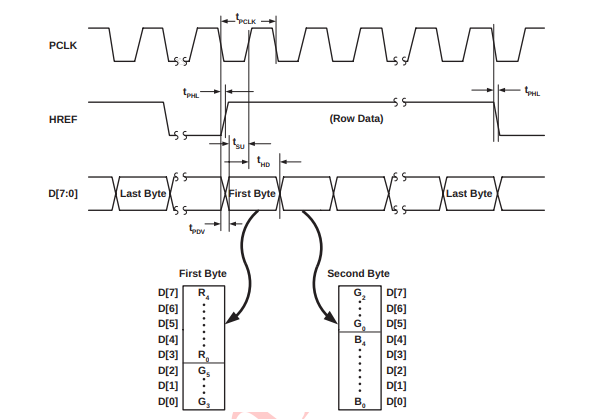
\includegraphics[width=0.85\textwidth]{gambar/rgb-565-signal.png}
		\caption{Timing keluaran data RGB565 pada kamera OV7670}
		\label{fig:rgb-565-signal}
	\end{figure}

	Gambar~\ref{fig:rgb-565-signal} menunjukkan urutan sinyal keluaran kamera
	OV7670 ketika menggunakan format RGB565. Pada format ini, satu piksel warna
	direpresentasikan dalam 16 bit, sehingga data piksel dikirim melalui dua
	tahap byte secara berurutan pada jalur data paralel kamera. Sinyal PCLK
	digunakan sebagai acuan pengambilan data, sedangkan HREF menunjukkan bahwa
	data pada baris citra sedang valid. Pola timing ini menjadi dasar pengujian
	sanitasi kamera karena logika penerima harus mengambil byte pada siklus yang
	tepat agar pasangan data RGB565 tidak tertukar atau bergeser. Gambar tersebut
	diadaptasi dari datasheet OV7670 yang menjelaskan hubungan antara PCLK, HREF,
	dan keluaran data piksel pada mode RGB565 \cite{OmniVision2006OV7670}.

    \subsection{Pengujian Sanitasi VGA}
	Pengujian sanitasi VGA dilakukan menggunakan pola warna sederhana. Pola ini membantu memastikan bahwa timing VGA dan jalur RGB bekerja secara benar sebelum tampilan dihubungkan dengan data yang berasal dari DDR.
	\begin{lstlisting}[language=Verilog, title={Kode Sanitasi VGA Verilog}, label={code:verilog-sanitize}]
case (h_count[9:7])
// White
3'd0: begin vga_r <= 4'hF;vga_g <= 4'hF;vga_b <= 4'hF;end
// Yellow
3'd1: begin vga_r <= 4'hF;vga_g <= 4'hF;vga_b <= 4'h0; end
// Cyan
3'd2: begin vga_r <= 4'h0;vga_g <= 4'hF;vga_b <= 4'hF; end
// Green
3'd3: begin vga_r <= 4'h0;vga_g <= 4'hF;vga_b <= 4'h0; end
// Magenta
3'd4: begin vga_r <= 4'hF;vga_g <= 4'h0;vga_b <= 4'hF; end
// Red
3'd5: begin vga_r <= 4'hF;vga_g <= 4'h0;vga_b <= 4'h0; end
// Blue
3'd6: begin vga_r <= 4'h0;vga_g <= 4'h0;vga_b <= 4'hF; end
// Black
default: begin vga_r  <= 4'h0;vga_g <= 4'h0;vga_b <= 4'h0; end
endcase
	\end{lstlisting}
    \subsection{Pengujian DDR}
	Pengujian DDR dilakukan untuk memastikan transaksi baca dan tulis melalui MIG dan AXI berjalan setelah proses kalibrasi selesai. Validasi dilakukan terhadap kestabilan akses alamat dan kesesuaian data yang ditulis dan dibaca kembali.
    \subsection{Pengujian Sistem Terintegrasi}
	Pengujian sistem terintegrasi dilakukan setelah blok CNN, kamera, DDR, dan VGA lulus pengujian dasar. Pendekatan bertahap ini digunakan agar kesalahan integrasi dapat ditelusuri berdasarkan blok yang sudah tervalidasi sebelumnya.

\section{Metode Evaluasi}
    \subsection{Evaluasi Akurasi}
	Evaluasi akurasi digunakan untuk menilai kesesuaian hasil klasifikasi terhadap
	label data uji dan sebagai pembanding antara baseline software dan implementasi
	hardware. Pada penelitian ini, evaluasi akurasi tidak hanya dinyatakan dalam
	bentuk nilai akurasi keseluruhan, tetapi juga dianalisis menggunakan
	\emph{confusion matrix}.

	\emph{Confusion matrix} digunakan karena mampu menunjukkan hubungan antara
	label sebenarnya dan label hasil prediksi untuk setiap kelas digit. Nilai pada
	diagonal utama menunjukkan jumlah data yang diklasifikasikan dengan benar,
	sedangkan nilai di luar diagonal menunjukkan kesalahan klasifikasi antar kelas.
	Dengan cara ini, evaluasi tidak hanya menjawab apakah model benar atau salah
	secara umum, tetapi juga menunjukkan kelas digit mana yang lebih sering tertukar
	dengan kelas lain.

	Penggunaan \emph{confusion matrix} penting pada penelitian ini karena model CNN
	diimplementasikan kembali dari Python ke Verilog dengan representasi
	fixed-point. Jika terjadi penurunan akurasi atau perubahan hasil prediksi,
	\emph{confusion matrix} dapat membantu melihat apakah perubahan tersebut
	terjadi merata pada seluruh kelas atau hanya dominan pada kelas tertentu.
	Analisis ini digunakan untuk menilai apakah hasil inferensi hardware masih
	konsisten terhadap baseline model Python.
    \subsection{Evaluasi Perbedaan Bit}
	Evaluasi perbedaan bit digunakan untuk melihat dampak representasi fixed-point
	terhadap nilai antara pada setiap blok CNN. Evaluasi ini penting karena
	kesalahan kecil pada layer awal dapat terakumulasi pada layer berikutnya.
	Pada penelitian ini, keluaran antara dari implementasi Verilog dibandingkan
	dengan keluaran baseline Python yang sudah dikonversi ke format fixed-point.
	Dengan demikian, pembandingan tidak dilakukan langsung antara nilai
	\emph{floating-point} dan nilai hardware, tetapi melalui representasi integer
	fixed-point yang sama.

	Pembacaan hasil dari Verilog memerlukan proses \emph{sign extension} karena
	data yang ditangkap dari simulasi atau hasil dump hardware dapat terbaca
	sebagai unsigned integer, padahal nilai aktivasi atau hasil akumulasi
	menggunakan representasi two's complement bertanda. Oleh karena itu, nilai
	unsigned perlu dikembalikan menjadi signed integer berdasarkan lebar bit yang
	digunakan pada masing-masing blok. Selain itu, keluaran Python juga dikonversi
	ke fixed-point dengan jumlah bit fraksi yang sama, yaitu $F=14$, agar
	perbandingan bit dilakukan pada skala numerik yang setara.

	Potongan kode yang digunakan untuk proses evaluasi tersebut ditunjukkan pada
	Listing~\ref{code:bit-difference-eval}. Fungsi \texttt{sign\_extend}
	digunakan untuk mengubah data unsigned two's complement menjadi signed integer
	sesuai lebar bit tertentu, sedangkan fungsi \texttt{python\_float\_to\_fixed}
	digunakan untuk mengubah keluaran \emph{floating-point} Python menjadi integer
	fixed-point. Mode pembulatan digunakan agar proses konversi mengikuti prinsip
	kuantisasi parameter yang digunakan pada implementasi model.

	\begin{lstlisting}[language=Python, title={Kode evaluasi perbedaan bit Python dan Verilog}, label={code:bit-difference-eval}]
def sign_extend(arr, bit_width):
    """
    Untuk mengubah unsigned two's complement menjadi signed integer.
    Contoh kalau ACT_SIZE = 24, maka bit_width = 24.
    """
    arr = arr.astype(np.int64)

    if bit_width is None:
        return arr

    sign_bit = 1 << (bit_width - 1)
    full_range = 1 << bit_width

    return np.where(arr >= sign_bit, arr - full_range, arr)


def python_float_to_fixed(arr, frac_bits=14, mode="round"):
    """
    Convert float Python ke fixed-point integer.
    """
    scale = 1 << frac_bits
    scaled = arr * scale

    if mode == "round":
        return np.round(scaled).astype(np.int64)

    elif mode == "trunc":
        return np.trunc(scaled).astype(np.int64)

    elif mode == "floor":
        return np.floor(scaled).astype(np.int64)

    else:
        raise ValueError("mode harus 'round', 'trunc', atau 'floor'")
	\end{lstlisting}

    \subsection{Evaluasi Latensi Inferensi}
	Evaluasi latensi inferensi dihitung berdasarkan jumlah siklus clock yang diperlukan sejak data masukan mulai diproses oleh blok CNN sampai keluaran klasifikasi tersedia. Pengukuran ini dilakukan karena sistem tidak hanya harus menghasilkan prediksi yang benar, tetapi juga harus mampu menghasilkan keluaran dalam batas waktu yang sesuai dengan kebutuhan \emph{real-time}. Pada implementasi sinkron di FPGA, waktu eksekusi lebih tepat dinyatakan berdasarkan jumlah siklus clock karena setiap tahap komputasi, pembacaan FIFO, operasi MAC, dan propagasi antarblok dikendalikan oleh sinyal clock.

	Latensi inferensi dihitung menggunakan Persamaan~\ref{eq:latensi-inferensi}. Nilai $N_{cycle}$ menyatakan jumlah siklus clock yang dibutuhkan untuk menyelesaikan satu proses inferensi, sedangkan $f_{clk}$ menyatakan frekuensi kerja clock sistem dalam satuan Hz.

	\begin{equation}
		T_{latency} = \frac{N_{cycle}}{f_{clk}}
		\label{eq:latensi-inferensi}
	\end{equation}

	Jika frekuensi clock dinyatakan dalam MHz, maka latensi dalam mikrodetik dapat dihitung menggunakan Persamaan~\ref{eq:latensi-inferensi-us}. Persamaan ini digunakan untuk memudahkan interpretasi hasil pengujian karena nilai latensi inferensi pada FPGA umumnya berada pada orde mikrodetik hingga milidetik.

	\begin{equation}
		T_{latency}(\mu s) = \frac{N_{cycle}}{f_{clk}(\text{MHz})}
		\label{eq:latensi-inferensi-us}
	\end{equation}

	Throughput dihitung sebagai jumlah inferensi yang dapat diselesaikan dalam satu detik. Untuk satu jalur inferensi tanpa pemrosesan paralel antar citra, throughput dapat diperoleh dari kebalikan latensi seperti ditunjukkan pada Persamaan~\ref{eq:throughput-inferensi}. Dengan demikian, semakin kecil jumlah siklus inferensi atau semakin tinggi frekuensi clock yang digunakan, semakin besar throughput yang dapat dicapai oleh akselerator.

	\begin{equation}
		Throughput = \frac{1}{T_{latency}} = \frac{f_{clk}}{N_{cycle}}
		\label{eq:throughput-inferensi}
	\end{equation}

	Apabila pengujian dilakukan untuk beberapa citra uji, throughput rata-rata dihitung menggunakan Persamaan~\ref{eq:throughput-rata-rata}. Nilai $N_{image}$ menyatakan jumlah citra yang diuji, sedangkan $T_{total}$ menyatakan total waktu yang dibutuhkan untuk menyelesaikan seluruh proses inferensi.

	\begin{equation}
		Throughput_{avg} = \frac{N_{image}}{T_{total}}
		\label{eq:throughput-rata-rata}
	\end{equation}

	Hasil latensi dan throughput kemudian digunakan untuk menilai apakah strategi implementasi yang dipilih, seperti pemotongan bit hasil MAC, penggunaan FIFO, dan algoritma prapemrosesan citra, masih memenuhi kebutuhan kecepatan sistem secara keseluruhan.
    \subsection{Evaluasi Penggunaan Resource FPGA}
	Evaluasi resource FPGA menilai penggunaan LUT, FF, BRAM, dan DSP pada CNN accelerator maupun sistem terintegrasi. Hasilnya digunakan untuk menganalisis trade-off antara paralelisme, time multiplexing, dan kelayakan implementasi.
    \subsection{Evaluasi Daya}
	Evaluasi daya menggunakan hasil estimasi implementasi untuk menilai kesesuaian sistem dengan motivasi embedded vision yang membutuhkan konsumsi daya rendah.
    \subsection{Evaluasi Tampilan Real Time}
	Evaluasi tampilan real-time dilakukan dengan melihat apakah jalur kamera, DDR, dan VGA mampu bekerja stabil ketika sistem dijalankan. Evaluasi ini melengkapi pengujian CNN karena sistem akhir tidak hanya berupa akselerator, tetapi sistem embedded vision end-to-end.

\section{Tahapan Pelaksanaan}
Tahapan pelaksanaan penelitian ini ditunjukkan pada
Gambar~\ref{fig:diagram-alir-penelitian}. Penelitian
diawali dengan studi literatur untuk memahami konsep
implementasi CNN pada
FPGA, teknik kuantisasi \emph{fixed-point}, serta
sistem pendukung seperti kamera, memori DDR, dan
tampilan VGA. Setelah itu, model CNN dikembangkan
terlebih dahulu menggunakan Python sebagai model acuan.
Model yang telah diperoleh kemudian dikonversi ke
representasi \emph{fixed-point} 16-bit agar lebih sesuai
dengan karakteristik komputasi FPGA. Tahap kuantisasi
ini divalidasi berdasarkan dua aspek, yaitu akurasi
model dan kebutuhan \emph{resource} FPGA, karena
implementasi CNN pada FPGA perlu mempertimbangkan
keseimbangan antara performa komputasi, penggunaan
sumber daya, dan ketelitian numerik
\cite{Solovyev2019FixedPointCNN, Jacob2018Quantization}.

Setelah model hasil kuantisasi dinilai memenuhi
kebutuhan, arsitektur CNN diimplementasikan ke dalam
Verilog. Hasil implementasi Verilog kemudian dibandingkan
dengan hasil model Python melalui pengujian
\emph{bit-difference} untuk memastikan bahwa proses
komputasi pada hardware tetap mengikuti model acuan.
Tahap berikutnya adalah pengujian dasar hardware menggunakan
\emph{debug} ILA untuk memastikan blok kamera, FIFO, DDR,
dan VGA dapat bekerja dengan benar sebelum dilakukan
integrasi sistem. Setelah seluruh blok tervalidasi, sistem
diintegrasikan menjadi alur lengkap mulai dari pengambilan
citra, pemrosesan CNN, hingga evaluasi hasil inferensi.

\begin{figure}[H]
	\centering
	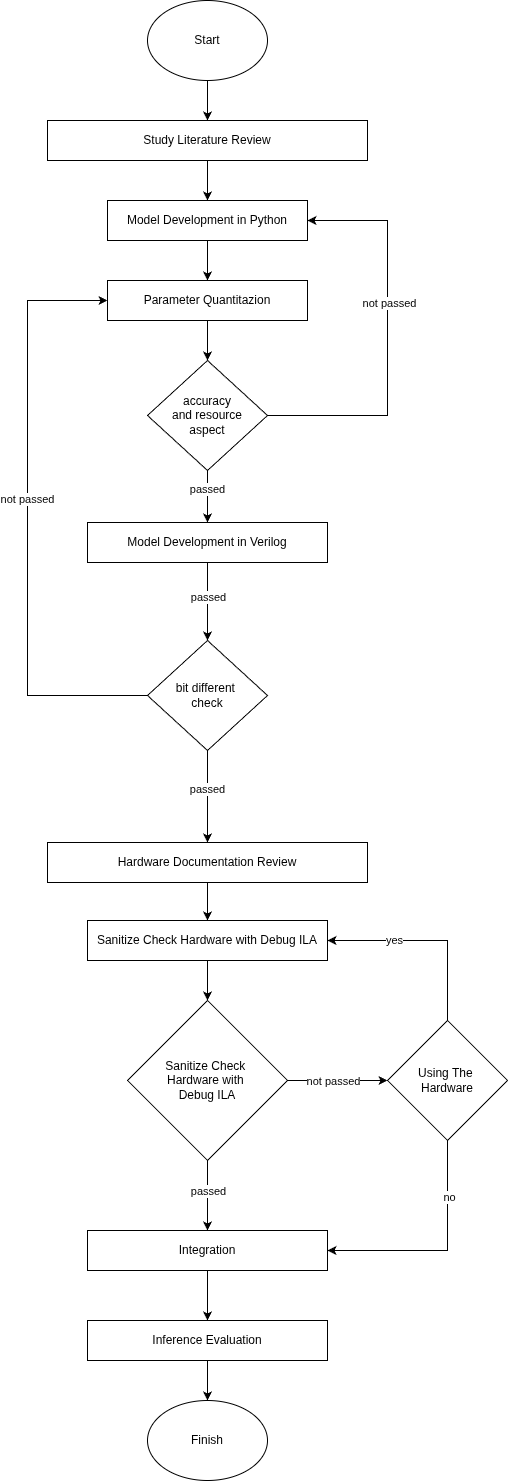
\includegraphics[width=0.45\textwidth]{gambar/diagram-alir-penelitian.png}
	\caption{Diagram Alir Penelitian}
	\label{fig:diagram-alir-penelitian}
\end{figure}

\section{Jadwal Kegiatan}
Penelitian dilaksanakan selama enam bulan, yaitu dari
Januari 2026 hingga Juni 2026 sebagaimana ditunjukkan pada
Tabel \ref{jadwal-penelitian}. Tahap studi literatur
dilakukan pada bulan pertama hingga bulan ketiga sebagai
dasar dalam penyusunan dan pengembangan penelitian.
Desain sistem dilaksanakan mulai bulan kedua hingga bulan
keenam dengan mengacu pada hasil studi literatur serta
penelitian terdahulu yang relevan. Pembuatan prototipe
dilakukan secara paralel dengan proses desain sistem pada
bulan keempat hingga bulan keenam dengan mempertimbangkan
kapasitas perangkat keras dan waktu penelitian yang tersedia.
Uji coba dan perbaikan sistem juga dilaksanakan pada periode
yang sama untuk mengevaluasi kinerja prototipe dan melakukan
penyempurnaan secara bertahap. Adapun penulisan skripsi
dilakukan pada bulan keenam sebagai tahap akhir penelitian.


\begin{table}[H]
	\centering
	\caption{Jadwal Penelitian.}
	\label{jadwal-penelitian}
	\begin{tabular}{|c|l|l|l|l|l|l|l|}
	\hline
	\multirow{2}{*}{No} & \multirow{2}{*}{Keterangan} & \multicolumn{6}{c|}{Bulan} \\ \cline{3-8}
						&                             & 1 & 2 & 3 & 4 & 5 & 6 \\ \hline
	1 & Studi literatur        & \cellcolor{gray} & \cellcolor{gray} & \cellcolor{gray} &                        &                        &                        \\ \hline
	2 & Desain                 &                    & \cellcolor{gray} & \cellcolor{gray} & \cellcolor{gray} & \cellcolor{gray} & \\ \hline
	3 & Pembuatan prototipe    &                    &                    &                    & \cellcolor{gray} & \cellcolor{gray} & \cellcolor{gray} \\ \hline
	4 & Uji coba dan perbaikan &                    &                    &                    & \cellcolor{gray} & \cellcolor{gray} & \cellcolor{gray} \\ \hline
	5 & Penulisan skripsi      &                    &                    &                    &                    &                    & \cellcolor{gray} \\ \hline
	\end{tabular}
\end{table}
